 %!TEX root = ./template-skripsi.tex
%-------------------------------------------------------------------------------
%                            BAB II
%               KAJIAN TEORI
%-------------------------------------------------------------------------------

\chapter{KAJIAN PUSTAKA} 

% \section{Related Work}

% \textit{\textbf{Bipartite Graph Partitioning}}: sebuah \textit{bipartite graph} yang terdiri dari dua set \textit{disjoint} dari titik-titik X dan Y yang tidak ada garis yang memiliki masing-masing \textit{end point} di dalam set yang sama. Masalah \textit{graph partitioning} secara umum adalah \textit{NP hard} untuk \textit{bipartite graph}, \textit{partitioning} teroptimasi dengan meminimalisir suatu \textit{global function}. Banyak algoritma klastering yang telah diajukan untuk melakukan \textit{partitioning} pada \textit{bipartite graph}. Algoritma \textit{Min-Max Cut} meminimalisir total bobot di antara klaster dan memaksimalkan total bobot di dalam klaster. \textit{Spectral Clustering} secara bersamaan mengklasterkan baris dan kolom dari \textit{adjacency matrix} dari suatu graf. Namun, \textit{spectral clustering} bisa gagal dalam beberapa kasus di mana dua \textit{bipartite graph} bersatu menjadi suatu \textit{tripartite graph} karena sifat keheterogenan dari titik-titik. Untuk mengatasinya, algoritm \textit{Consistent Bipartite Graph Co-partitioning (CBGC)} diajukan. \textit{CBGC} mengaplikasikan \textit{semi-definite programming (SDP)} untuk mengatasi \textit{star-structured high order heterogeneous data} dengan merepresentasikan mereka sebagai beberapa graf \textit{bipartite} dan mengoptimalkan \textit{global function} untuk mencari pemotongan terbaik. Namun, CBGC hanya bisa mengatasi \textit{binary clustering problem} dan tidak cocok untuk pekerjaan multiklastering.

% \textit{\textbf{Low Rank Matrix Approximation}}: \textit{Low rank matrix approximation} adalah suatu permasalahan terkait aproksimasi \(m x n\) matriks \(A\) dengan matriks rank \(k\) yang lain, di mana \(k\) lebih kecil dibandingkan \(m\) dan \(n\). Metode tradisional seperti \textit{Singular Value Decomposition (SVD)} bisa digunakan untuk mencari matriks tersebut, tetapi waktu komputasinya biasanya sangat lama yaitu \(Omin\{mn^2, nm^2\}\).

% Sebelumnya, metode \textit{near-optimal} \textit{low rank matrix approximation} mulai menjadi populer. Jika kita \textit{denote} \(A_k\) sebagai aproksimasi optimal rank \(k\) dari matriks \(A\), tujuannya adalah untuk mencari \textit{near-optimal} matriks \(A_k^*\) yang meminimalisir error \(e\):

% \begin{equation}
%     ||A - A_k^*|| \leq ||A - A_k|| + e
% \end{equation}

% Dekomposisi \(CUR\) merupakan salah satu algoritma yang aproksimasi \(A\) dengan \(A = CUR\), di mana \(C\) adalah matriks \textit{consisting} dari angka-angka kecil dari kolom \(A\), \(R\) adalah matriks \textit{consisting} dari angka-angka kecil di baris \(A\), dan \(U\) adalah matriks \textit{appropriately defined low dimensional encoding}. Dengan demikian, \(CUR\) matriks dekomposisi menyediakan \textit{dimensionally reduced low rank approximation} menjadi data matriks orisinil \(A\) yang terdiri dari angka kecil dari kolom sekarang dan baris dari matriks original. Secara waktu baik linear dan konstan dari algoritma \(CUR\) telah diusulkan menjadi mengaproksimasikan matriks berukuran besar secara efisien.Namun, sejak baris dan kolom dipilih secara random, \(CUR\) tidak bisa memastikan akan matriks yang simetris. Hal ini membuatnya tidak cocok untuk kasus \textit{bipartite graph} karena \textit{biparite graph} membutuhkan beban matriks yang selalu simetris.

\section{Representasi Bipartite Graph}

Mendefinisikan suatu graf \(G = (V, E, W)\) sebagai suatu set dari titik-titik \(V\) dan hubungan mereka dengan garis \(E\), dengan \(W\) sebagai bobot dari garis-garis tersebut. Sebagai contoh, \(w_{ij}\) sebagai bobot dari garis di antara titik \(i\) dan \(j\).

Graf $G$ disebut \textit{bipartite} jika mengandung dua kelas titik $X$ dan $Y$ sebagai berikut $V = X \cup Y$ dan $X \cap Y = \emptyset$ setiap garis $e_{ij} \in E$ memiliki \textit{endpoint} $i$ di dalam $X$ dan \textit{endpoint} lain $j$ di dalam $Y$. Biasanya, $X$ dan $Y$ merujuk kepada perbedaan tipe objek dan $E$ merepresentasikan relasi antara keduanya. Di dalam konteks representasi dokumen, $X$ merupakan suatu set dokumen, sedangkan $Y$ adalah \textit{terms} dan $w_{ij}$ merupakan banyaknya \textit{term} $j$ yang muncul di dalam dokumen $i$. Perlu dicatat bahwa \textit{weighted adjacency matrix} $W$ untuk \textit{bipartite graph} selalu simetris. Sebagai contoh, gambar berikut adalah \textit{undirected bipartite graph} dengan 4 dokumen dan 5 \textit{term}.

\begin{figure}[h]
    \centering
    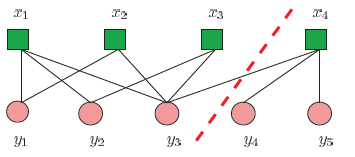
\includegraphics[width=0.75\textwidth]{gambar/Bipartite Graph.PNG}
    \caption{Suatu \textit{bipartite graph} \(X\) dan \(Y\) \cite{song2008autotag}}
    \label{gambar:bipartite_graph}
\end{figure}

\subsection{Normalisasi dan Aproksimasi}

Normalisasi biasanya digunakan pertama kali untuk bobot matriks \(W\) untuk mengeliminasi \textit{bias}. Jalur yang paling lurus untuk menormalisasikan \(W\) adalah normalisasi baris yang tidak mengambil akun dari simetri pada \(W\). Namun, untuk memahami simetri pada \(W\), Song dkk menggunakan \textit{normalized graph Laplacian} untuk aproksimasi \(W\). \textit{Normalized Laplacian} \(L(W)\) sebagai berikut.

\begin{align*}
L(W)_{i j} = \begin{cases}1-\frac{w_{i j}}{d_{i}} & \text { jika } i=j, \\ -\frac{w_{i j}}{\sqrt{d_{i} d_{j}}} & \text { jika } i \text { dan } j \text { terhubung } \\ 0 & \text { selain itu, }\end{cases}
\end{align*}

di mana \(d_i\) adalah \textit{degree} luar dari titik \(i\), pada persamaan $d_{i}=\sum w_{i j}, \forall j \in$ $V$. Kemudian, kita bisa mendefinisikan matriks diagonal \(D\) di mana $D_{ii} = d_i$. Oleh karena itu, \textit{normalize Laplacian} dapat direpresentasikan sebagai berikut. 

\begin{equation}
\label{normalize_laplacian}
    L(W) = D^{(-1/2)}WD^{(-1/2)}
\end{equation}

Untuk \textit{dataset} berskala besar seperti situs \textit{corpora} dan koleksi gambar, spasi fitur mereka biasanya mengandung jutaan vektor dengan dimensi yang sangat tinggi (contohnya, \(x\) = $10^6$, y = $10^7$). Oleh karena itu, biasanya ini sering diinginkan untuk mencari \textit{low rank matrix $W$ komplemen} untuk aproksimasi $L(W)$ dengan tujuan untuk mengurangi biaya komputasi, mengekstrak korelasi, dan menghapus \textit{noise}. Metode dekomposisi matriks tradisional misalnya adalah \textit{Single Value Decomposition} dan \textit{eigenvalue decomposition}, membutuhkan waktu \textit{superlienar} untuk perkalian matriks vektor jadi biasanya mereka tidak menggunakannya sampai pengaplikasian di dunia nyata.

Untuk \textit{symmetric low rank apporiximation}, di sini menggunakan algoritma Lanczos yang secara iteratif mencari nilai eigen dan vektor eigen dari matriks persegi. Diberikan $n$ x $n$ \textit{sparse symmetric matrix} $A$ dengan nilai eigen:

\begin{equation}
\label{lambda_lambda}
    \lambda \geq ... \geq \lambda_n \geq 0
\end{equation}

Algoritma Lanczos menghitung $k$ x $k$ \textit{symmetric tridiagonal matrix} $T$, yang nilai eigennya mengaproksimasi nilai eigen dari $A$, dan vektor eigen dari $T$ bisa digunakan untuk mengaproksimasi vektor eigen $A$, dengan $k$ lebih kecil dibandingkan $n$. Dengan kata lain, $T$ yaitu:

\begin{equation}
\label{frobenius_norm}
    ||A - T||_F \leq e||A||_F
\end{equation}

di mana $||.||_F$ denotasi \textit{Frobenius norm}, dengan \(e\) sebagai variabel terkendali. Sebagai contoh, untuk menangkap \(95 \% \) varians dari \(A\), \(e\) diatur sebagai 0.05.

\subsection{Bipartite Graph Partitioning}

Untuk melakukan multi-klastering pada \textit{bipartite graph}, \cite{song2008autotag} menggunakan algoritma \textit{Spectral Recursive Embedding (SRE)}. Secara esensial, \textit{SRE} digunakan untuk menkontruksi \textit{partition} dengan meminimalisir normalisasi dari total pada bobot garis di antara pasangan yang tidak cocok pada suatu garis, misalnya \(min_{\Pi(A,B)}Ncut(A,B)\), di mana \(A\) dan \(B\) adalah pasangan yang cocok dalam partisi dengan $A^c$ dan $B^c$ menjadi yang lain. Normalisasi varian dari \textit{edge cut} \(Ncut(A,B)\) didefinisikan sebagai berikut.

\begin{equation}
    \label{n_cut}
    Ncut(A,B) = \frac{cut(A,B)}{W(A,Y)+W(X,B)} + \frac{cut(A^c,B^c)}{W(A^c,Y)+W(X,B^c)},
\end{equation}

di mana

\begin{equation}
\begin{split}
\label{cut_ab}
    cut(A,B) &= W(A,B^c) + W(A^c, B) \\
             &= \sum_{i \in A, j \in B^c}{} w_{ij} + \sum_{i \in A^c, j \in B}{} w_{ij},
\end{split}
\end{equation}

Rasional dari \(Ncut\) tidak hanya mencari partisi dengan perpotongan garis kecil, tetapi juga mepartisinya sepadat mungkin. Ini berguna untuk aplikasi dari \textit{tagging document} di mana dokumen dengan setiap partisi secara ideal berfokus kepada satu topik spesifik. Sebagai hasil, semakin padat suatu partisi, semakin baik yang dokumen relevan dan \textit{tag} terkelompokkan bersamaan.

\subsection{Dengan Cluster Node Ranking}

\cite{song2008autotag} mendefinisikan dua pengukuran baru \textit{N-Precision} dan \textit{N-Recall} untuk \textit{node ranking}. \textit{N-Precision} dari titik \(i\) merupakan jumlah total dari bobot pada garis yang terkoneksi kepada titik dalam klaster yang sama, dibagi dengan jumlah total dari bobot garis yang ada di dalam klaster. Label klaster \(i\) sebagai \(C(i)\),

\begin{equation}
\label{n_precision}
    np_i=\frac{\sum_{j=1}^{n}w_{ij}\Pi[C(j) = C(i)]}{\sum_{j,k=1}^{n}w_{jk}\Pi[C(j) = C(k) = C(i)]},j,k\neq i,
\end{equation}

Untuk graf tidak berbobot, persamaan di atas setara dengan banyaknya garis yang berasosiasi dengan titik \(i\) di dalam klaster \(C(i)\), dibagi dengan total garis yang ada di dalam klaster \(C(i)\). Secara umum, \textit{N-precision} mengukur seberapa pentingnya titik pada suatu klaster, di dalam perbandingan dengan titik lain. Dalam konteks pada suatu dokumen, klasternya adalah suatu set topik dari dokumen dan bobot dari titik-titik kata menunjukkan frekuensi dari kata-kata yang muncul pada topik tersebut. Dengan \textit{cluster determined}, \textit{denominator equation} bersifat konstan, jadinya semakin banyak bobot yang dimiliki pada suatu titik, semakin penting pula.

Kontrasnya, \textit{N-recall} digunakan untuk menghitungkan probabilitas posterior dari titik \(i\) pada klaster yang diberikan dan \textit{inverse} pembagian dari garis i yang berasosiasi dengan klasternya.

\begin{equation} \label{n_recall}
    nr_i= \frac{|E_i|}{\sum_{j=1}^{n}w_{ij}\Pi[C(j) = C(i)]}.
\end{equation}

Hal tersebut merupakan bukti bahwa \textit{N-Recall} selalu tidak kurang dari satu. Semakin lebar \textit{N-Recall}, maka semakin mungkin bahwa kata tersebut berasosiasi dengan suatu topik yang spesifik.

Diberikan \(np_i\) dan \(nr_i\), kita akan melakukan estimasi dari peringkat \(i\):

\begin{equation}\label{rank_i}
\begin{split}
    Rank_i = \begin{cases} \exp(-\frac{1}{r(i)^2}) , & r(i) \neq 0, \\
    0, & r(i) = 0, \\
    \end{cases}
    \textbf{di mana}\, r(i) = (np_i) * log(nr_i)
\end{split}
\end{equation}


Berdasarkan persamaan di atas, fungsi perangkingan dari \cite{song2008autotag} merupakan pengganti yang dihaluskan yang proporsional untuk presisi titik (\textit{node precision}) dan \textit{recall}, hasilnya terjamin berada di kisaran \textit{range (0, 1)}.

Potensi pengalikasian dari metodologi \textit{bipartite graph node ranking} termasuk interpetasi relasi dokumen dan \textit{author} yaitu menentukan relasi sosial (misal "\textit{hub}" dan "\textit{authority}") dari \textit{author} di dalam satu topik penelitian yang sama, dan mencari representatif dokumen dari suatu topik. Di sini, mereka mengaplikasikan \textit{framework} ini untuk melakukan rekomendasi \textit{tag} dengan \textit{ranking node} yang merepresentasikan \textit{tag} pada setiap klaster.
\begin{figure}[H]
    \centering
    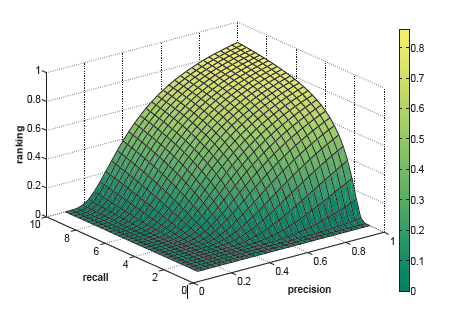
\includegraphics[width=0.75\textwidth]{gambar/Smoothed Ranking Function.PNG}
    \caption{Smoothed Ranking Function \cite{song2008autotag}}
    \label{gambar:smoothed_ranking_function}
\end{figure}

\section{Online Tag Recommendation}

Suatu dokumen biasanya mengandung beberapa kata dan beberapa \textit{tag} yang dibuat oleh \textit{user}. Hubungan antara dokumen, kata-kata, dan \textit{tag} bisa direpresentasikan dengan gambar dua \textit{bipartite graph} yang akan ditunjukkan oleh gambar setelah ini. 

Graf yang berbobot dapat ditulis dsebagai berikut
\begin{equation} \label{w_ab}
    W = \begin{pmatrix}
0 & A & 0\\
A^T & 0 & B\\
0 & B^T & 0
\end{pmatrix}
\end{equation}
di mana \(A\) dan \(B\) sebagai matriks-matriks inter-relasi antara \textit{tag} dengan dokumen dan dokumen dengan kata-kata.

\begin{figure}[H]
    \centering
    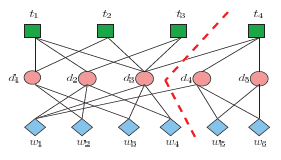
\includegraphics[width=0.75\textwidth]{gambar/Two Bipartite Graph of Tag Document Word.PNG}
    \caption{Dua bipartite graph dari dokumen-dokumen, kumpulan kata, dan kumpulan tag. \cite{song2008autotag}}
    \label{gambar:smoothed_ranking_function}
\end{figure}

Diberikan suatu representasi matriks, pendekatan lurus untuk \textit{tag} rekomendasi adalah dengan melihat kemiripannya antara dokumen \textit{query} dan dokumen \textit{training} dengan fitur-fitur kata, kemudian lakukan \textit{top ranked tags} dari dokumen yang paling mirip. Pendekatan ini biasanya direferensikan sebagai filter kolaborasi. Namun, pendekatan ini tidaklah efisien untuk skenario dunia nyata. Untuk mengambil kelebihan dari algoritma \textit{node ranking}, Song dkk menggunakan \textit{Possion Mixture Model (PMM)} yang secara efisien menentukan sampel \textit{membership} sebaik klastering kata-kata dengan makna yang mirip. Sebelum melakukan  \textit{mixture model}, di sini terdapat rangkuman algoritma yang digunakan untuk rekomendasi \textit{tag} di dalam Algoritma 1. (\cite{song2008autotag})

\begin{algorithm} [H]
\caption{Online Tag Recommendation \citep*{song2008autotag}}\label{alg:online_tag_recommendation}
\begin{algorithmic}
\State 1: \textbf{Input} $(\mathcal{D}, S, T), K, M, L$ \\
$\quad$ Kumpulan dokumen: $\mathcal{D}=\left\{\mathcal{D}_{1}, \ldots, \mathcal{D}_{m}\right\}$ \\
$\quad$ \textit{Word vocabulary}: $S=\left\{S_{1}, \ldots, S_{k}\right\}$ \\
$\quad$ \textit{Tag vocabulary}: $T=\left\{T_{1}, \ldots, T_{n}\right\}$ \\
$\quad$ banyaknya klaster: $K \in \mathbb{R}$ \\
$\quad$ banyaknya komponen-komponen: $M \in \mathbb{R}$ \\
$\quad$ banyaknya klaster-klaster kata: $ L \in \mathbb{R} $ \\
\textit{\textbf{Offline Computation}} \\
2: Menunjukkan bobot terdekat matriks W seperti persamaan (\ref{w_ab}) \\
3: Normalisasi $W$ menggunakan \textit{Normalized Laplacian} persamaan (\ref{normalize_laplacian}) \\
4: Komputasi \textit{low rank approximation matrix} menggunakan Lanczos: \\
$\quad \tilde{W} \simeq L(W)=Q_{k} T_{k} Q_{k}^{T}$ \\
5: Partisi $\tilde{W}$ ke dalam klaster K menggunakan SRE, 
$\quad \tilde{W}=\left\{\tilde{W}_{1}, \ldots, \tilde{W}_{K}\right\}$ \\
6: Tandai label ke dalam setiap dokumen $\mathcal{D}_{j}, j \in\{1, \ldots m\}$ \\
$\quad C\left(\mathcal{D}_{j}\right) \in\{1, \ldots, K\}$ \\
7: Hitung \textit{node rank} $Rank(T)$ untuk setiap tag $T_{i, k}$ di dalam klaster \\
$k, i \in\{1, \ldots, n\}, k\{1, \ldots, K\} \quad$ persamaan (\ref{rank_i}) \\
8: Buat \textit{Poisson Mixture Model} untuk $(\tilde{B}, C(\mathcal{D}))$ dengan $M$ komponen-komponen dan $L$ klaster kata-kata, di mana $\tilde{B}$ denotasi matriks inter-relationship pada suatu dokumen-dokumen dan kata-kata di dalam $\tilde{W}$ persamaan (\ref{w_ab})\\
\textit{\textbf{Online Recommendation}} \\
9: Untuk setiap dokumen tes $\mathbb{Y}$, kalkulasikan posterior probabilitas \\
$P(C=k \mid D=\mathbb{Y})$ di dalam setiap klaster $k$, dan denotasi membership pada $\mathbb{Y}$ sebagai $C(\mathbb{Y})=\{c(\mathbb{Y}, 1), \ldots, c(\mathbb{Y}, K)\}$ persamaan (\ref{bayes_rules}) \\
10: Tag rekomendasi berdasarkan perangkingan pada tag, yaitu \textit{joint probability} pada tag-tag $T$ dan dokumen $Y$, $R(T, \mathbb{Y})$ persamaan (\ref{rank_tag}) \\
\end{algorithmic}
\end{algorithm}

Dua tahap \textit{framework} ini bisa diinterpretasikan sebagai prosedur \textit{unsupervised-supervised learning}. Saat tahap \textit{offline learning stage}, titik-titik akan dipartisi ke dalam klaster-klaster menggunakan \textit{unsupervised learning}, label klaster dipasangkan kepada \textit{document node} sebagai \textit{class label} mereka, dan tag akan diberikan \textit{rank} di dalam setiap klaster. \textit{Mixture model} kemudian dibangun berdasarkan distribusi dari dokumen-dokumen dan kata-kata. Di dalam \textit{online recommendation stage}, suatu dokumen diklasifikasikan ke dalam \textit{predefined cluster} yang telah didapatkan di dalam tahap pertama oleh Naive Bayes jadi \textit{tag} tersebut bisa direkomendasikan di pengurutan secara terbalik dari rank mereka. Untuk menghindari kebingungan, \cite{song2008autotag} akan merujuk kepada klaster yang diinginkan dengan mempartisi algoritima di dalam tahap pertama sebagai \textit{classess} di dalam sesi selanjutnya. (\cite{song2008autotag})

\subsection{Two-Way Poisson Mixture Model}

\cite{song2008autotag} mengusulkan untuk menggunakan \textit{Poisson Mixture Model} untuk mengestimasi distribusi data pada vektor dokumen sebab algoritma tersebut  cocok digunakan dibandingkan \textit{standard Poissons} dengan memproduksi estimasi lebih baik pada data varians dan cukup mudah untuk estimasi parameter. Akan tetapi, itu membutuhkan waktu untuk mencocokkan data latihan. Algoritma ini efisien untuk memprediksi label kelas dari dokumen baru setelah model tersebut selesai dibuat. Karena stabilitas numerikal pada pendekatan statistika ini, biasanya hasilnya dapat diandalkan. Sejak hanya estimasi probabilitas yang dilibatkan, ini dapat diandalkan untuk proses secara \textit{real-time}.

Namun, pendekatan tradisional \textit{unsupervised learning} dari \textit{mixture model} tidak selalu diandalkan untuk menghadapi klasifikasi dokumen. Mempertimbangkan kelemahan dan tingginya dimensi pada matriks \textit{document-word} di mana kebanyakan masukkan berupa 0 dan 1, model bisa saja gagal untuk memprediksi distribusi yang benar (yaitu \textit{probability mass faunction}) pada komponen yang berbeda. Sebagai hasilnya, klasterisasi kata adalah langkah yang diperlukan sebelum mengestimasi komponen-komponen di dalam model. Di sini akan dilakukan \textit{two-way Poisson Mixture Model} untuk secara bersamaan melakukan \textit{cluster word feature} dan klasifikasi dokumen.

\begin{figure}[H]
    \centering
    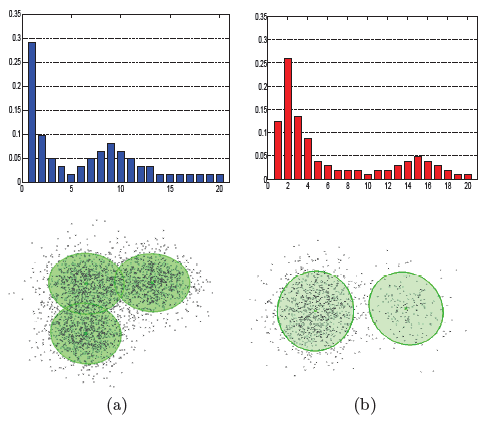
\includegraphics[width=0.75\textwidth]{gambar/Poisson Distribution in Two Cluster.PNG}
    \caption{Distribusi Poisson dalam dua klaster. Bagian atas menggambarkan histogram dari \textit{mixture components}. Bagian bawah menggambarkan hasil dari klasifikasi \textit{mixture model}. Bagian (a) \textit{three component mixtures} dan bagian (b) \textit{two component mixtures} \cite{song2008autotag}}
    \label{gambar:distribution_poisson}
\end{figure}

Diberikan suatu dokumen \(D = \{D_1, ..., D_p\}\), di mana \(p\) adalah dimensi, distribusi pada vektor dokumen di setiap kelas dapat diestimasikan dengan menggunakan \textit{parametric mixture model}.

kelas label \(C = \{1,2,...,K\},\) kemudian
\begin{equation}
\label{poisson_mixture_model_1}
    P(D = d | C = k) = \sum_{m=1}^{M}\pi_m\Pi(F(m) = k) \prod_{j=1}^{p}\phi(d_j|\lambda_{j,m}),
\end{equation}

di mana \(\pi_m\) adalah \textit{prior probability} dari komponen \(m\), dengan \(\sum_{m=1}^{M}\pi_m = 1\).\(\Pi(F(m) = k)\) adalah fungsi indikator yaitu apakah komponen \(m\) milik kelas \(k\), dan \(\phi\) merujuk kepada \textit{probability mass function} dari distribusi Poisson, \(\phi(d_j|\lambda_{j,m}) = e^{-\lambda_{j,m}}\lambda_{j,m^{d_j}}/ d_j\)!.

Pada jalur ini, setiap kelas adalah \textit{mixture model} dengan distribusi yang multivariasi dengan memiliki variabel yang mengikuti distribusi Poisson. Gambar 2.4 menunjukkan histogram pada dua \textit{mixture} yang bisa dianggap sebagai pmf dari dua \textit{Poisson mixture}.

Asumsi \cite{song2008autotag} terkait setiap kelas, kata-kata pada dokumen yang berbeda memiliki parameter Poisson yang setara, saat dokumen-dokumen di dalam kelas yang berbeda, kata-kata bisa saja mengikuti perbedaan distribusi Poissson. Untuk mempersimpel, \cite{song2008autotag} mengasumsi bahwa semua kelas memiliki nomor yang dari klaster-klaster kata. \textit{Denote} \(l = \{1,,,,L\}\) untuk menjadi klaster-klaster kata, kata-kata yang sama klaster kata \(m\) akan memiliki parameter yang sama yaitu \(\lambda_{i,m} = \lambda_{j,m} = \lambda_{l,m}\) untuk \(c(i,k) = c(j,k)\) di mana \(c(i,k)\) \textit{denote} label klaster pada kata \(i\) di dalam kelas \(k\). Berarti, persamaan sebelumnya dapat dipermudah menjadi (dengan $L \ll p$):

\begin{equation}
\label{poisson_mixture_model_2}
    P(D = d | C = k) \propto \sum_{m=1}^{M}\pi_m\Pi(F(m) = k) \prod_{l=1}^{L}\phi(d_{k,l}|\lambda_{l,m}),
\end{equation}

\subsubsection{Estimasi Parameter}

Dengan kelas yang dideterminasi, berikutnya masukkan algoritma EM untuk mengestimasi parameter Poisson \(\lambda_{l,m}, l \in \{1, ..., L\}, m \in \{1, ..., M\}\), \textit{prior of mixture component} \(\pi_m\), dan indeks klaster kata \(c(k,j) \in \{1, ..., L\},k \in \{1, ..., K\}, j \in \{1, ..., p\}\).

Estimasi \textit{E-step} \textit{posterior probability} \(p_{i,m}\) sebagai berikut.

\begin{equation}
\label{e_step}
p_{i, m} \propto \pi_{m}^{(t)} \mathbb{II}(C(i)) \prod_{j=1}^{p} \theta\left(d(i, j) \mid \tilde{\lambda}_{m, i, j}^{(t)}\right) 
\end{equation}

\textit{M-step} menggunakan \(p_{i,m}\) untuk memaksimalkan \textit{objective function}


\begin{equation}
\label{m_step}
\begin{aligned}
&\quad L\left(\pi_{m}^{(t+1)}, \tilde{\lambda}_{m, l}^{(t+1)}, c^{(t+1)}(k, j) \mid \pi_{m}^{(t)}, \tilde{\lambda}_{m, l}^{(t)}, c^{(t)}(k, j)\right) \\
&=\max \sum_{i=1}^{n} \sum_{m=1}^{M} p_{i, m} \log \left(\pi_{m}^{(t+1)} \mathbb{I}(C(i)) \prod_{j=1}^{p} \theta\left(d(i, j) \mid \tilde{\lambda}_{m, i, j}^{(t+1)}\right)\right),
\end{aligned}
\end{equation}


dan \textit{update} parameter


\begin{equation}
\label{update_parameter_pi}
\pi_{m}^{(t+1)}=\frac{\sum_{i=1}^{n} p_{i, m}}{\sum_{m^{\prime}=1}^{M} \sum_{i=1}^{n} p_{i, m^{\prime}}}, \\ \\ 
\end{equation}
\begin{equation}
\label{update_parameter_lambda}
\tilde{\lambda}_{m}^{(t+1)}=\frac{\sum_{i=1}^{n} p_{i, m} \sum_{j} d(i, j) \mathbb{I}(C(i))}{|d(i, j)| \sum_{i=1}^{n} p_{i, m}},
\end{equation}


di mana $|d(i,j)|$ denotasi bilangan dari $j$ di dalam komponen $l$.

Setelah $\tilde{\lambda}_{m}^{(t+1)}$ telah diperbaiki, indeks klaster kata $c^{(t+1)}(k, j)$ bisa ditemukan dengan melakukan \textit{linear search} pada semua komponen-komponen:

$$
c^{(t+1)}(k, j)=\arg \max _{l} \sum_{i=1}^{n} \sum_{m=1}^{M} \log \left(d(i, j) \mid \tilde{\lambda}_{m, l}^{(t+1)}\right)
$$

(\cite{song2008autotag})

\subsection{Tag Recommendation for New Documents}

Normalnya, label kelas $C(d_{t})$ dari suatu dokumen baru $d_t$ ditentukan oleh $\hat{C}(x)=\arg \max _{k} P\left(C=k \mid D=d_{t}\right)$. Namun, di kasus ini, \cite{song2008autotag} determinasi \textit{mixed membership} pada suatu dokumen dengan menkalkulasi \textit{posterior probabilities} pada suatu kelas dengan $\sum_{k=1}^{K} P\left(C=k \mid D=d_{t}\right)=1$. Mengaplikasikan persamaan (2.12) dan \textit{Bayes Rule},

\begin{equation}
\label{bayes_rules}
    \begin{split}
        P (C = k | D = d_t) 
        &= \frac{P(D = d_t | C = k) P(C=k)}{P(D=d_t)} \\
        &= \frac{\sum_{m=1}^{M} \pi_{m} \mathbb{II}(F(m)=k) \prod_{l=1}^{L} \phi(d_{k, l} \tilde{\lambda}_{l, m}) P(C=k)}{P(D=d_{t})}
    \end{split}
\end{equation}

di mana $P(C = k)$ adalah \textit{prior probabilites} dari kelas $k$ dan set seragam. Akhirnya, probabilitas untuk setiap \textit{tag} $T_{i}, i \in$ $\{1, \ldots, n\}$ diasosiakan dengan sampel adalah

\begin{equation}
\label{rank_tag}
    \begin{split}
        R(T_{i}, d_{t})
        &= P(T=T_{i}|D=d_{t}) \\
        &= Rank_{T_{i}} * P(C=x|D=d_{t})
    \end{split}
\end{equation}

Dengan perangkingan \textit{tag} dari terbesar ke terkecil pada probabilitas mereka, \textit{top ranked tags} dipilih untuk rekomendasi. (\cite{song2008autotag})

\section{Mixture Model}

Salah satu \textit{Mixture Model} yang  biasa dipakai yaitu \textit{Gaussian Mixture Model} (\textit{GMM}), \textit{GMM} adalah suatu \textit{parametric probability density function} yang merepresentasikan \textit{weighted sum} dari kepadatan komponen \textit{Gaussian}. Biasanya, \textit{GMM} digunakan sebagai \textit{parametric model} dari distribusi probabilitas pada pengukuran yang kontinu. Parameter \textit{GMM} diestimasi dari data latih menggunakan algoritma \textit{Expectation-Maximization} (\textit{EM}).

\textit{Gaussian Mixture Model} adalah \textit{weighted sum} dari \textit{M} kepadatan komponen \textit{Gaussian} dengan persamaan sebagai berikut.

\begin{equation}
    \label{eq:gaussian_mixture_model}
    p(x|\lambda) = \sum_{i=1}^{M} w_i g(x|\mu_i, \Sigma_i)
\end{equation}

Di mana x adalah $D$ \textit{dimensional continuous} vektor data, $w_i$, i = 1, ...,$M$ adalah bobot mikstur, dan $g(x|miu_i, \Sigma_i)$, $i$ = 1,...,$M$ adalah kepadatan komponen \textit{Gaussian}. Kepadatan komponen \textit{Gaussian} adalah sebagai berikut.

\begin{equation}
    \label{eq:component_gaussian_densities}
    g(x|\mu_i, \Sigma_i) = \frac{1}{(2\Phi)^{D/2}|\Sigma_i|^{1/2}}
    exp\{-\frac{(x-\mu_i)'\Sigma_i^{-1}(x-\mu_i)}{2}\}
\end{equation}

dengan $\mu_i$ sebagai \textit{mean vector} dan $\sigma_i$ sebagai matriks kovarian. \textit{Mixture Weights} memenuhi persamaan $\sum_{i=1}^{M}w_i = 1$.

Beberapa parameter tersebut dikumpulkan menjadi persamaan berikut.

\begin{equation}
    \label{eq:lambda_gaussian_mixture_model}
    \lambda = \{w_i, \mu_i, \sigma_i\} \\
    i = 1, ..., M
\end{equation}

Pada tahap selanjutnya adalah menghitung \textit{Maximum Likelihood Parameter}. Diberikan data latih berupa vektor-vektor dan konfigurasi \textit{GMM}. Dari sini akan dilakukan estimasi dari parameter \textit{GMM} $\lambda$. Metode paling populer dalam menentukan ini adalah estimasi \textit{Maximum Likelihood}.

Tujuan \textit{Maximum Likelihood} adalah mencari parameter model yang memaksimalkan \textit{likelihood} pada GMM dari data latih yang diberikan. Untuk setiap $T$ \textit{training vector} $X$ = $\{x_1,...,x_T\}$, \textit{GMM likelihood}, asumsikan antar vektor adalah independen, maka sebagai berikut.

\begin{equation}
    \label{eq:gmm_likelihood}
    p(X|\lambda) = \prod_{t=1}^{T} p(x_t|\lambda)
\end{equation}

Sayangnya, persamaan ini adalah fungsi tidak linear dari parameter $\lambda$ dan tidak mungkin untuk melakukan pemaksimalan secara langsung. Namun, parameter \textit{Maximum Likelihood} dapat diestimasikan dengan cara iteratif dengan menggunakan algoritma \textit{Expectation-maximization} (\textit{EM}).

Ide dasar dari algoritma \textit{EM} adalah memulai model awal $\lambda$ untuk mengistmasi model baru $\tilde{\lambda}$ lalu menjadi $p(X|\tilde{\lambda}) \geq p(X|\lambda)$. Model baru akan menjadi model awal untuk iterasi selanjutnya dan proses tersebut akan berlanjut sampai batas tertentu yang ditetapkan. Model awal biasanya \textit{derived} dengan menggunakan \textit{VQ estimation}. (\cite{reynolds_gaussian_mixture_model})

Dalam setiap iterasi \textit{EM}, formula reestimasi selanjutnya akan digunakan untuk meningkatkan nilai \textit{likelihood}.

\textit{Mixture Weights}
\begin{equation}
    \label{eq:gmm_em_mixture_weight}
    \tilde{w}_i = \frac{1}{T} \sum_{t=1}^{T}Pr(i|x_t, \lambda)
\end{equation}

\textit{Means}
\begin{equation}
    \label{eq:gmm_em_means}
    \tilde{\mu}_i = \frac{\sum_{t=1}^{T}Pr(i|x_t, \lambda) x_t}{\sum_{t=1}^{T}Pr(i|x_t, \lambda)} 
\end{equation}

\textit{Varians}
\begin{equation}
    \label{eq:gmm_em_varians}
    \tilde{\sigma}^2_i = \frac{\sum_{t=1}^{T}Pr(i|x_t, \lambda) x_t^2}{\sum_{t=1}^{T}Pr(i|x_t, \lambda)}  - \tilde{\mu_i^2}
\end{equation}

Kemudian \textit{posterior probability} untuk komponen $i$ sebagai berikut.

\begin{equation}
    \label{eq:gmm_em_posterior_probability}
    Pr(i|x_t, \lambda) = \frac{w_i g(x_t|\mu_i, \Sigma_i)}{\sum_{k=1}^{M}w_k g(x_t|\mu_i, \Sigma_i)}
\end{equation}

Perbedaan antara Distribusi Gaussian dengan Distribusi Poisson sebagai berikut.

\begin{figure}[H]
    \centering
    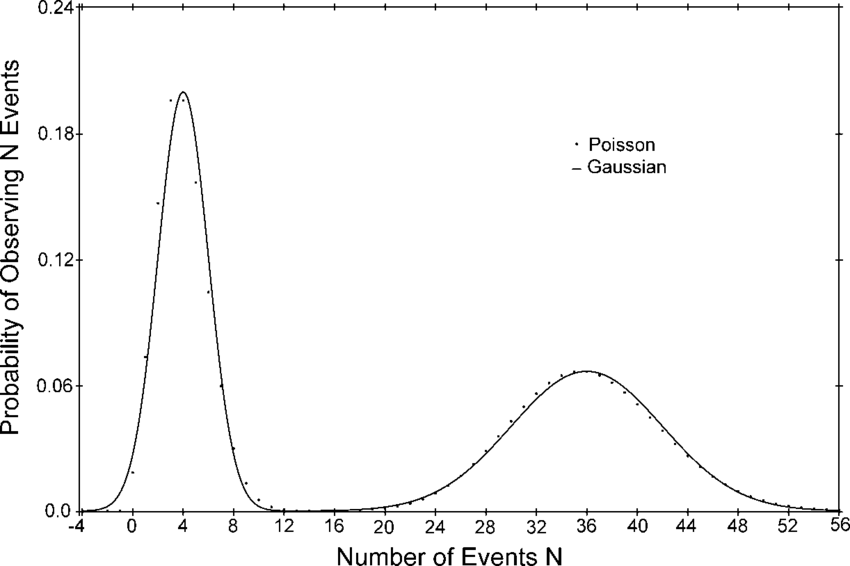
\includegraphics[width=0.50\textwidth]{gambar/Difference-between-Gaussian-and-Poisson-distributions-Graph-shows-two-Poisson-and-two.png}
    \caption{Perbedaan antara Distribusi Gaussian dengan Distribusi Poisson \cite{rzeszotarski_physics_tutorial}}
    \label{gambar:flowchart_automatic_tag}
\end{figure}

% \section{Lanczos Bidiagonalization dan SVD}

% Untuk mencari vektor singular baik kiri maupun kanan, diperlukan algoritma \textit{Lanczos Bidiagonalization}. Dalam algoritma tersebut terdapat, terdapat matriks penting seperti $U^T A V = B$ 

% \begin{align*}
%     U &= [u_1, ..., u_m] \\
%     V &= [v_1, ..., v_n] \\
%     U^TU &= I_m \\
%     V^TV &= I_n
% \end{align*}

% B adalah matriks \textit{bidiagonalization} sebagai berikut.

% \begin{equation*}
% B=\left[\begin{array}{ccccc}
% \alpha_{1} & \beta_{1} & & \ldots & 0 \\
% & \alpha_{2} & \beta_{2} & & \vdots \\
% &  & \alpha_{3} & \ddots & \\
% \vdots  & & & \ddots & \beta_{k-1} \\
% 0 & \ldots  & & & \alpha_{k}
% \end{array}\right] .
% \end{equation*}

% \begin{algorithm}[H]
% \caption{\textit{Lanczos Bidiagonalization Algorithm} \citep*{golub_matrix_computation_3_edition}}\label{alg:lanczos_bidiagonalization}
% \begin{algorithmic}
% \State $v_1 =$  given unit 2-norm n-vector ; $p_0 = v_1$
% % \State 
% \State $\beta_0 = 1$ ; $k = 0$ ; $u_0 = 0$
% % \State 
% \While{$\beta \neq 0$}
% \State $v_{k+1} = p_k/\beta_k$
% \State $k = k + 1$
% \State $r_k = Av_k - \beta_{k-1}u_{k-1}$
% \State $\alpha_k = \Vert r_k \|_2$
% \State $u_{k} = r_k/\alpha_k$
% \State $p_{k} = A^Tu_k-\alpha_kv_k$
% \State $\beta_k = \Vert p_k \|_2$
% \EndWhile
% \end{algorithmic}
% \end{algorithm}

% Dengan algoritma seperti itu, akan didapat hasil-hasil dari vektor singularnya.
